%%% Notes on Single stellar population production of N %%% 

\providecommand{\main}{..} 
\documentclass[\main/notes.tex]{subfiles} 

\begin{document} 
\begin{center} 
\textbf{{\Large Single Stellar Population Production of Nitrogen}} 
\end{center} 

\noindent 
{\Large \textit{Production Timescales Relative to Fe}} 
\par\noindent 
Using~$y_\text{N}^\text{CC} = 5\times10^{-4}$, the AGB star yields of N from 
the FRUITY database~\citep{Cristallo2011}, and supernova yields of Fe as in 
\citet{Johnson2020} and~\citet{Weinberg2017} (i.e.~$y_\text{Fe}^\text{CC}$ = 
0.0012 and~$y_\text{Fe}^\text{Ia}$~= 0.0017),~\textbf{what is the net 
production of N and Fe as a function of stellar population age and 
metallicity?} 
\par 
Figure~\ref{fig:n_vs_fe_ssp} shows the net production of N and Fe as a function 
of stellar population age and metallicity. Since Fe has metallicity-independent 
yields under these assumptions, it's plotted with only one curve, whereas N has 
different production timescales at different metallicities. In general, the 
CCSN yields of N under these assumptions make up a substantially larger 
fraction of the N production than the CCSN yields of Fe does for its 
production. This means that the characteristic timescales for N production are 
significantly shorter than for Fe. 
\par
The AGB yields of N are also significantly weighted toward high masses such 
that even at solar metallicity,~$\gtrsim$90\% of the N production is complete 
by the time the population is~$\tau$~= 1 Gyr old. Although the fractional 
yields are higher for more massive AGB stars, this does not mean that the 
total N produced in low-mass AGB stars is lower than that produced by high mass 
AGB stars due to the steep nature of the initial mass function. In a window of 
progenitor mass [$m$,~$m + dm$] at a metallicity~$Z$, the total mass of N 
produced is given by: 
\begin{equation} 
dm_\text{N} = y(m|Z)m\frac{dN}{dm} = y(m|Z)\xi m^{1 - \alpha} 
\end{equation} 
where~$\alpha$~is the power-law index of the IMF. If the production at two 
masses~$m_1$~and~$m_2$~are comparable, then the scaling of the yield~$y$~with 
progenitor mass can be derived: 
\begin{subequations}\begin{align} 
dm_\text{N}|_{m = m_1} &= dm_\text{N}|_{m = m_2} \\ 
\implies y(m_1|Z) \xi m_1^{1 - \alpha} &= y(m_2|Z) \xi m_2^{1 - \alpha} \\ 
\implies \frac{y(m_1|Z)}{y(m_2|Z)} &= \left(\frac{m_1}{m_2}\right)^{\alpha - 1} 
\end{align}\end{subequations} 

\begin{figure}[t] 
\centering 
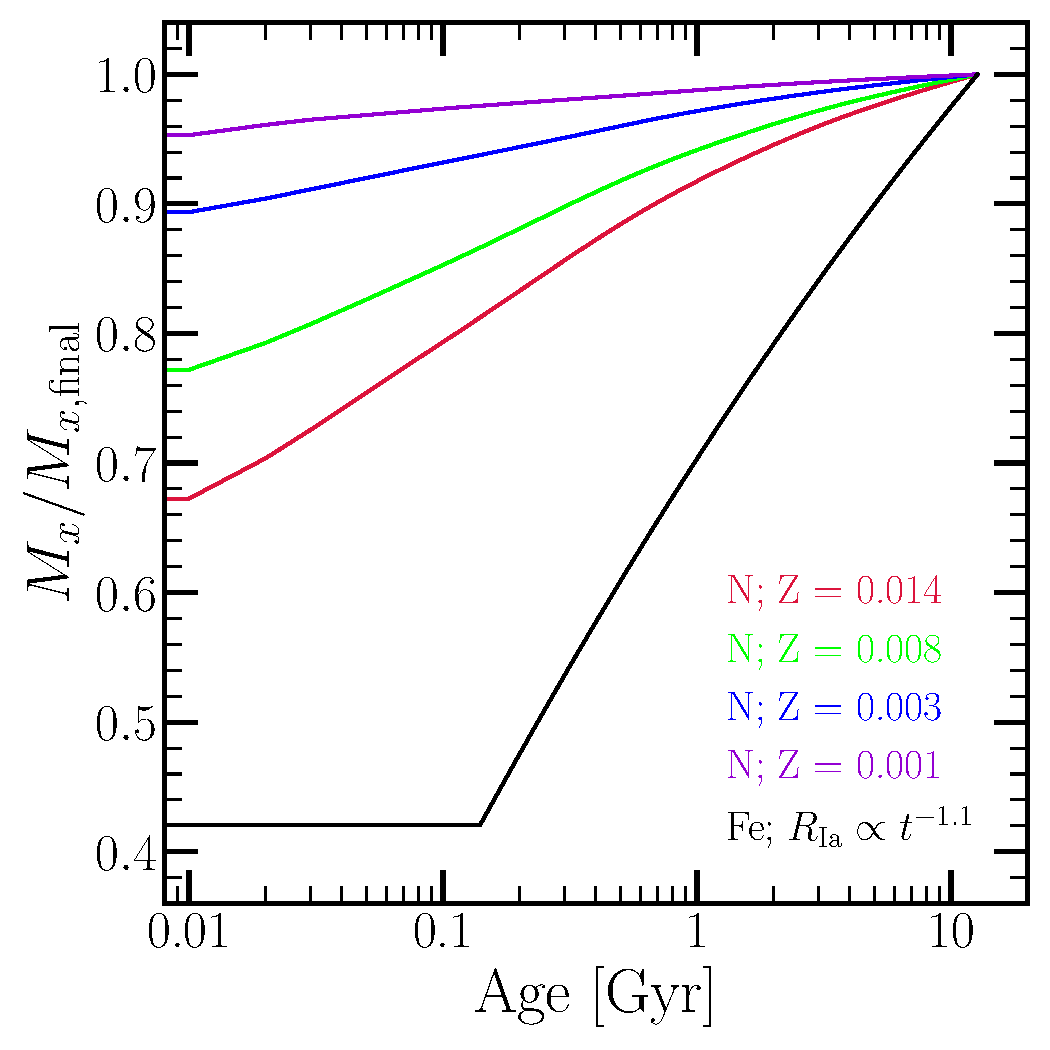
\includegraphics[scale = 0.5]{\main/ssp/n_vs_fe_ssp.pdf} 
\caption{Net mass of N (colored lines) and Fe (black) as a function of stellar 
population age and metallicity (color-coded according to legend for N), in 
units of the mass produced at~$\tau$~= 12.2 Gyr. } 
\label{fig:n_vs_fe_ssp} 
\end{figure} 

If the yield~$y$~scales with~$m^{-\gamma}$ and the IMF-integrated mass 
production is to be mass-independent, then~$\gamma = 1 - \alpha$~= -1.3. Only 
when~$y \propto m^{1.3}$ will the IMF-integrated contribution of high mass 
stars be comparable to that of low-mass stars. The weight of low-mass stars 
increases with increasing~$\gamma$, and conversely for high-mass stars with 
decreasing~$\gamma$. Based on these investigations of the~\citet{Cristallo2011} 
yields (see~\texttt{latex/yields/yields.pdf}), it appears 
that~$\gamma \approx$~-1 for nitrogen (if anything else, the~$y-m$ relation 
appears to me that it might be slightly sub-linear), indicating that the 
IMF-integrated production is marginally dominated by low-mass stars. 

\twolineskip 
{\Large \textit{How can the production be dominated by high-mass stars if the 
IMF-integrated yields are dominated by low-mass stars?}} 
To understand this, it is enlightening to consider the scenario in which the 
production of some element~$x$~in AGB stars is time-independent. That is, 
\begin{equation} 
\dot{M}_x^\text{AGB} = \text{constant} 
\end{equation} 
Under this assumption, in any time interval from~$\tau$~to~$\tau + d\tau$, the 
amount of production of some element~$x$~is always the same. This corresponds 
to an idealized scenario in which stars of all masses contribute equally to 
enrichment when stellar lifetimes are taken into account. The question then 
becomes,~\textbf{what is the required dependence of the AGB yield on mass at a 
given metallicity for the production rate to be constant?} For this calculation, 
we'll assume the IMF, lifetime, and yield scale with progenitor stellar mass 
$m$~in the following way: 
\begin{subequations}\begin{align} 
\frac{dN}{dm} \propto m^{-\alpha} \\ 
\tau \propto m^{-\beta} \\ 
y \propto m^{-\gamma} 
\end{align}\end{subequations} 
where to answer this question we will need to calculate the appropriate value 
of~$\gamma$. 
\par 
The rate of production of some element~$x$~can be expressed according to: 
\begin{equation} 
\dot{M}_x^\text{AGB} = y(m_\text{to}|Z) M_\star \dot{h} 
\end{equation} 
where~$y(m_\text{to}|Z)$~is the yield at the main sequence turnoff mass at some 
metallicity~$Z$,~$M_\star$~is the total initial mass of the progenitor stellar 
population, and~$\dot{h}$~is the time-derivative of the~\textit{main sequence 
mass fraction} (see~\citet{Johnson2020}, or section 3 of VICE's science 
documentation\footnote{
	\url{https://vice-astro.readthedocs.io/en/latest/science_documentation/SSPs/index.html}
}). In detail, VICE takes into account post main-sequence lifetimes by simply 
inflating the lifetime~$\tau$ by some amount (10\% by default), but for the 
purposes of this calculation, I'm assuming it to be zero. It is defined by: 
\begin{equation} 
h = \ddfrac{
	\int_l^{m_\text{to}} m \frac{dN}{dm} dm 
}{
	\int_l^u m \frac{dN}{dm} dm 
}
\end{equation} 
where~$l$~and~$u$~are the lower and upper mass limits of star formation, 
respectively, and~$dN/dm$~is the IMF. Taking the time-derivative of~$h$~may 
appear non-trivial, but it is simplified greatly by the usage of the chain 
rule and the fundamental theorem of calculus. Conventiently, the demoninator of 
$h$~is simply the initial mass of the stellar population and is 
time-independent; for ease, I'll denote it here simply as~$M_\star$. 
\begin{subequations}\begin{align} 
\dot{h} &= M_\star^{-1} \frac{d}{dm_\text{to}} 
\left(\int_l^{m_\text{to}} m\frac{dN}{dm} dm\right) 
\frac{dm_\text{to}}{d\tau} 
\\ 
&= M_\star^{-1} m_\text{to} \frac{dN}{dm}\Big|_{m_\text{to}} 
\frac{dm_\text{to}}{d\tau} 
\\ 
&\propto M_\star^{-1} m_\text{to}^{1 - \alpha} \frac{d}{d\tau}(\tau^{-1/\beta}) 
\\ 
&\propto M_\star^{-1} m_\text{to}^{1 - \alpha} \frac{-1}{\beta} 
\tau^{-(1 + \beta)/\beta} 
\\ 
&\propto M_\star^{-1} \tau^{(\alpha - 1) / \beta} \frac{-1}{\beta} 
\tau^{-(1 + \beta)/\beta} 
\\ 
&\propto M_\star^{-1} \frac{-1}{\beta} \tau^{(\alpha - 2 - \beta)/\beta} 
\end{align}\end{subequations} 
Therefore, under this formalism, the main sequence mass fraction should 
decrease monotonically with time (as expected) according to 
$\dot{h}~\sim~\tau^{(\alpha - 2 - \beta) / \beta}$. 
\par 
Next, if the yield~$y$~scales with~$m_\text{to}^{-\gamma}$, then it should 
scale with time according to~$y~\sim~\tau^{\gamma/\beta}$. Plugging all of this 
in yields the following time-dependence for the AGB enrichment rate: 
\begin{subequations}\begin{align} 
\dot{M}_x^\text{AGB} &\sim \tau^{\gamma/\beta} 
\tau^{(\alpha - 2 - \beta) / \beta} 
\\ 
&= \tau^{(\alpha + \gamma - 2 - \beta) / \beta} 
\end{align}\end{subequations} 
and if the enrichment rate is to be a constant, the power-law index must be 
equal to zero: 
\begin{equation} 
\alpha + \gamma - 2 - \beta = 0 \implies \gamma = 2 + \beta - \alpha 
\end{equation} 
If~$\alpha$~= 2.3 and~$\beta$~= 3.5, as adopted in VICE, then~$\gamma$~= 3.2. 
If all stellar masses are to contribute equally to the AGB enrichment rate when 
lifetimes are taken into account such that the rate is constant, then the 
yields must increase sharply with decreasing stellar mass. I note that the 
high value of~$\gamma$~is truly a consequence of the high value of~$\beta$ 
($2 - \alpha$~= -0.3). Under this parameterization, for higher values of 
$\gamma$, the AGB enrichment rate increases with time as the yields of low-mass 
stars become more and more important. For lower values, the production rate 
falls with time due to the lifetimes of low-mass stars preventing them from 
producing yields quickly enough to maintain a constant production rate. This 
is an indication that even though the IMF-integrated AGB stars yields of N are 
marginally weighted toward low-mass AGB stars, the amount which is produced on 
the order of a hubble time will be dominated by high mass stars unless the 
yields have a very strong, inverse dependence on progenitor stellar mass. 

\biblio  

\end{document} 

